\question[3]
Two roads meet at right angles and are $a$~\si{\meter} and $b$~\si{\meter} wide, respectively, as shown in Figure~\ref{fig:two-roads}. Sign posts are positioned at $A$ and $C$. It's known that $A$, $B$ and $C$ are colinear. Show that $AC$ has length $a\sec(\theta) + b\csc(\theta)$.

\begin{figure}[h]
	\centering
	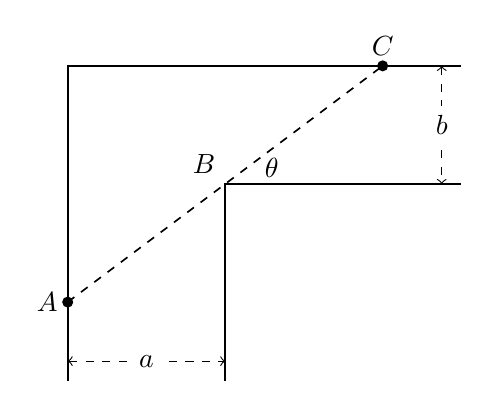
\begin{tikzpicture}
	\coordinate (RTL) at (0,0);
	\coordinate (RTR) at (5,0);
	\coordinate (RBL) at (0,-4);
	\coordinate (RBR) at (2,-4);
	\coordinate (RMR) at (5,-1.5);
	\coordinate (A) at (0,-3);
	\coordinate (B) at (2,-1.5);
	\coordinate (C) at (4,0);
	\draw[
		semithick,
	]
	(RBL) -- (RTL) -- (RTR);
	
	\draw[
		semithick,
	]
	(RBR) -- (B) node[anchor=south east] {$B$} -- (RMR);
	\draw[
		semithick,
		dashed,
	]
	(A) node[anchor=east] {$A$} -- (C) node[anchor=south] {$C$};
	\draw (B) node[above right, xshift=2.5ex, yshift=-.25ex] {$\theta$};
	\draw[
		dashed,
		<->,
	]
	(0,-3.75) -- node[midway,fill=white] {$a$~\si{\meter}} (2,-3.75);
	\draw[
		dashed,
		<->,
	]
	(4.75,0) -- node[midway,fill=white] {$b$~\si{\meter}} (4.75,-1.5);
	\fill[
		black,
	]
	(A) circle (2pt)
	(C) circle (2pt)
	;		
	\end{tikzpicture}
	\caption{The intersection of two roads.}
	\label{fig:two-roads}
\end{figure}

\begin{EnvFullwidth}
\begin{solutionorgrid}[4in]
\begin{center}
	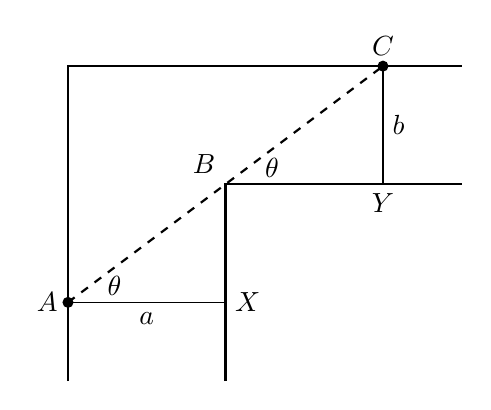
\begin{tikzpicture}
	\coordinate (RTL) at (0,0);
	\coordinate (RTR) at (5,0);
	\coordinate (RBL) at (0,-4);
	\coordinate (RBR) at (2,-4);
	\coordinate (RMR) at (5,-1.5);
	\coordinate (A) at (0,-3);
	\coordinate (B) at (2,-1.5);
	\coordinate (C) at (4,0);
	\coordinate (X) at (2,-3);
	\coordinate (Y) at (4,-1.5);
	\draw[
		thick,
	]
	(RBL) -- (RTL) -- (RTR);
	\draw[
		thick,
	]
	(RBR) -- (B) node[anchor=south east] {$B$} -- (RMR);
	\draw[
		thick,
		dashed,
	]
	(A) node[anchor=east] {$A$} -- (C) node[anchor=south] {$C$};
	\draw (B) node[above right, xshift=2.5ex, yshift=-.25ex] {$\theta$};
	\draw (A) node[above right, xshift=2.5ex, yshift=-.25ex] {$\theta$};
	\draw[
		-,
	]
	(A) -- node[midway, below] {$a$~\si{\meter}} (X);
	\draw[
		-,
	]
	(C) -- node[midway, right] {$b$~\si{\meter}} (Y);
	\fill[
		black,
	]
	(A) circle (2pt)
		(C) circle (2pt)
	;
	\draw (X) node[right] {$X$};
	\draw (Y) node[below] {$Y$};
	\end{tikzpicture}
\end{center}
If $\angle CBY = \theta$, then $\angle BAX = \theta$ and
\[
	\cos(\theta) = \frac{a}{AB},\qquad \sin(\theta) = \frac{b}{BC}.
\]
So,
\begin{align*}
	AB &= \frac{a}{\cos(\theta)} & BC &= \frac{b}{\sin(\theta)} \\
	&= a\sec(\theta), & &= b\csc(\theta).
\end{align*}
Now, $AC = AB + BC$, so $AC = a\sec(\theta) + b\csc(\theta)$, as required.
\end{solutionorgrid}
\end{EnvFullwidth}
